\chapter{Pruebas}
\label{cap:pruebas}

\section{Módulo primero de encadenamiento entre preguntas y respuestas}
Veamos algunos ejemplos de cómo funciona el primer acercamiento a un chatbot inteligente que pregunta con algo de sentido. A continuación se muestra la primera pregunta y la respuesta del interrogado:
\begin{itemize}
	\item[] IA: ¿Quiénes son las personas más importantes de tu vida?
	\item[] Tú: Mi familia y concretamente mis padres y mi hermano
\end{itemize}

En la siguiente texto de salida por consola se muestra el análisis que hace el módulo de cálculo de la mejor siguiente pregunta:

\begin{verbatim}

Maxima coincidencia de lemas hasta ahora: 0
Pregunta elegida hasta ahora: ¿Cuál es tu sexo?

Posible pregunta: ¿Hay algún momento que te gustaría volver a vivir?
Lemas de la posible pregunta: {'volver', 'vivir', 'momento', 'gustar'}
Lemas de la respuesta anterior: {'familia', 'padre', 'hermano'}
Lemas que coinciden: 0
-----------------------------------------------
Maxima coincidencia de lemas hasta ahora: 0
Pregunta elegida hasta ahora: ¿Cuál es tu sexo?

Posible pregunta: ¿Dónde viviste cuando eras pequeño?
Lemas de la posible pregunta: {'pequeño', 'vivistar'}
Lemas de la respuesta anterior: {'familia', 'padre', 'hermano'}
Lemas que coinciden: 0
-----------------------------------------------
Maxima coincidencia de lemas hasta ahora: 0
Pregunta elegida hasta ahora: ¿Cuál es tu sexo?

Posible pregunta: ¿Has vivido en algún lugar diferente cuando eras pequeño?
Lemas de la posible pregunta: {'lugar', 'pequeño', 'vivir'}
Lemas de la respuesta anterior: {'familia', 'padre', 'hermano'}
Lemas que coinciden: 0
-----------------------------------------------
Maxima coincidencia de lemas hasta ahora: 0
Pregunta elegida hasta ahora: ¿Cuál es tu sexo?

Posible pregunta: ¿Cómo se llaman tus padres?
Lemas de la posible pregunta: {'padre', 'llamar'}
Lemas de la respuesta anterior: {'familia', 'padre', 'hermano'}
Lemas que coinciden: 1
-----------------------------------------------
Maxima coincidencia de lemas hasta ahora: 1
Pregunta elegida hasta ahora: ¿Cómo se llaman tus padres?

Posible pregunta: ¿Si tienes hermanos, cómo se llaman?
Lemas de la posible pregunta: {'llamar', 'tener', 'hermano'}
Lemas de la respuesta anterior: {'familia', 'padre', 'hermano'}
Lemas que coinciden: 1
-----------------------------------------------
Maxima coincidencia de lemas hasta ahora: 1
Pregunta elegida hasta ahora: ¿Cómo se llaman tus padres?

Posible pregunta: ¿Cómo era la casa dónde viviste de pequeño?
Lemas de la posible pregunta: {'pequeño', 'casa', 'vivistar'}
Lemas de la respuesta anterior: {'familia', 'padre', 'hermano'}
Lemas que coinciden: 0
\end{verbatim}

%\begin{figure}[h]
	%\centering
	%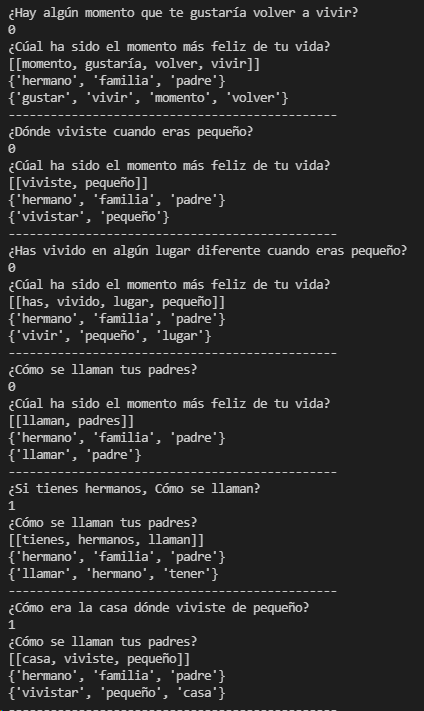
\includegraphics[scale=0.35]{Imagenes/Vectorial/modulo_encadenamiento_preguntas_respuestas_analisis}
	%\caption{}
	%\label{fig:moduloencadenamientopreguntasrespuestasanalisis}
%\end{figure}

En el texto podemos observar el análisis de varias posibles preguntas. La separación entre preguntas se marca con una fila de guiones. En cada apartado nos encontramos con la posible pregunta, después el número de lemas que han coincidido en preguntas anteriores, la pregunta que hasta el momento va ganando como candidata a ser preguntada, las palabras más relevantes de la posible pregunta entre corchetes, los lemas de la respuesta entre llaves y los lemas de la posible pregunta entre llaves. Las tres primeras preguntas no serán elegidas como candidatas a ser preguntadas porque no coincide ningún lema de la respuesta con los lemas de la posible pregunta, es decir, no mejora el número de coincidencias. Cuando llega a la cuarta pregunta, ``¿Cómo se llaman tus padres?'' va a encontrar una coincidencia de tal forma:

\begin{itemize}
	\item[] Lemas de la respuesta: \hspace{2cm} \{hermano, familia, padre\} 
	\item[] Lemas de la posible pregunta: \hspace{0.8cm} \{llamar, padre\}
\end{itemize}

Como podemos observar el lema ``padre'' coincide en ambas, es decir, en esta posible pregunta encontramos una coincidencia. Como el número de coincidencias es mejor que 0, la pregunta candidata ``¿Cuál ha sido el momento más feliz de tu vida?'' se sustituye por la pregunta ``¿Cómo se llaman tus padres?''. Es por esto que cuando analizamos el resto de posibles preguntas, no encontramos ninguna que sea mejor porque no superan el número de coincidencias en lemas. En conclusión, esta será la siguiente pregunta que se le plantee al usuario, la cual tiene relación con la que se había hecho anteriormente. 

\section{Módulo primero de clasificación de respuestas en etapas de vida y en sentimientos}

\begin{verbatim}
	Mi abuela se murio en 1998: 
	{'POSITIVO': 0.000133998051751405, 'NEGATIVO': 0.00039583168108947575, 'NEUTRO': 0.9994701743125916}
	['neutro']
	Mi mejor recuerdo es el del nacimiento de mi hijo: 
	{'POSITIVO': 0.0003367967437952757, 'NEGATIVO': 0.9894788861274719, 'NEUTRO': 0.010184396989643574}
	['negativo']
	Tengo 23 años: 
	{'POSITIVO': 0.016445694491267204, 'NEGATIVO': 0.0031412760727107525, 'NEUTRO': 0.980413019657135}
	['neutro']
	Me dolió muchísimo cuando me rompí una pierna: 
	{'POSITIVO': 0.0006958534941077232, 'NEGATIVO': 0.9989858269691467, 'NEUTRO': 0.0003183614171575755}
	['negativo']
	Mi hermano y yo nos pasabamos las tardes haciendo puzzles: 
	{'POSITIVO': 2.354631942580454e-05, 'NEGATIVO': 0.9972598552703857, 'NEUTRO': 0.0027166458312422037}
	['negativo']
	Durante la infancia estuvimos viviendo en Moratalaz: 
	{'POSITIVO': 0.051713500171899796, 'NEGATIVO': 0.9064642786979675, 'NEUTRO': 0.041822321712970734}
	['negativo']
	Mi pareja sufrió depresión después del parto: 
	{'POSITIVO': 2.2260337573243305e-05, 'NEGATIVO': 0.9954761862754822, 'NEUTRO': 0.004501543939113617}
	['negativo']
\end{verbatim}

\begin{verbatim}
	Mi abuela se murio en 1998: 
	{'POSITIVO': 0.09926079958677292, 'NEGATIVO': 0.9007392525672913}
	['negativo']
	Mi mejor recuerdo es el del nacimiento de mi hijo: 
	{'POSITIVO': 0.992607593536377, 'NEGATIVO': 0.007392475381493568}
	['positivo']
	Tengo 23 años: 
	{'POSITIVO': 0.9999983310699463, 'NEGATIVO': 1.6568293403906864e-06}
	['positivo']
	Me dolió muchísimo cuando me rompí una pierna: 
	{'POSITIVO': 2.0322097043390386e-05, 'NEGATIVO': 0.9999797344207764}
	['negativo']
	Mi hermano y yo nos pasabamos las tardes haciendo puzzles: 
	{'POSITIVO': 0.9681606888771057, 'NEGATIVO': 0.031839337199926376}
	['positivo']
	Durante la infancia estuvimos viviendo en Moratalaz: 
	{'POSITIVO': 0.9882893562316895, 'NEGATIVO': 0.011710633523762226}
	['positivo']
	Mi pareja sufrió depresión después del parto: 
	{'POSITIVO': 0.07562904059886932, 'NEGATIVO': 0.9243709444999695}
	['negativo']
\end{verbatim}



